% Provenance (never printed): old premiere S material on the lithosphere and the
% asthenosphere (chemical and mechanical layers, the low-velocity zone, the
% geotherm, isostasy); see sources/book2/PROVENANCE.md. S speeds from
% figdata/grade-11/prem_profiles.py (part upper), the geotherm and the solidus
% from geotherm_solidus.py, the elevations from hypsometry.py (ETOPO1).
% Glacial rebound belongs to g12; lithostatic pressure (term) to g12.
\chapter{Litosfer dan Astenosfer}\label{ch:g11:lithosphere-asthenosphere}

Sembilan persepuluh gunung es terletak di bawah air: es itu mengapung karena
massa jenisnya sedikit lebih kecil daripada laut, dan ia tenggelam ke dalam air
sampai air yang didesaknya sama beratnya dengan seluruh gunung es itu. Jajaran
pegunungan berperilaku dengan cara yang hampir sama. Di bawah pegunungan yang
paling tinggi, kerak hampir dua kali lebih tebal daripada biasanya, dan sebagian
besar kerak tambahan itu tersembunyi di bawahnya, seperti es di bawah garis
air. Tetapi gunung es mengapung di zat cair, sedangkan mantel di bawah jajaran
pegunungan adalah batuan padat. Bab ini menunjukkan bagaimana zat padat dapat
berperilaku seperti fluida yang di atasnya kulit luar Bumi mengapung, dan apa
kulit itu.
% ledger: usgs:ice-density, karplus:tibet-moho, cm95:crust

\begin{recall}
Bumi mempunyai kerak, mantel, dan inti (Buku 1, kelas 6). \omterm{def:g11:seismic-structure:moho}{Moho}, di dasar kerak,
terletak rata-rata sekitar \qty{41}{km} di bawah permukaan benua dan beberapa
kilometer di bawah dasar samudra; kecepatan seismik dan massa jenis diketahui
pada setiap kedalaman dari \omterm{def:g11:seismic-structure:reference-model}{model acuan Bumi}
(\cref{ch:g11:seismic-structure}). Batuan makin panas seiring kedalaman, sekitar
25 sampai \qty{30}{\celsius} per kilometer di dekat permukaan (Buku 1, kelas 6).
Benda yang mengapung di zat cair mendesak zat cair yang beratnya sama dengan
beratnya sendiri, dan tekanan di dasar suatu kolom bahan adalah berat kolom itu
dibagi luasnya (buku-buku fisika).
\end{recall}
% ledger: cm95:crust, usgs:crust-thickness, usgs:gradient-29 (Book 1 rows)

\begin{omfigure}
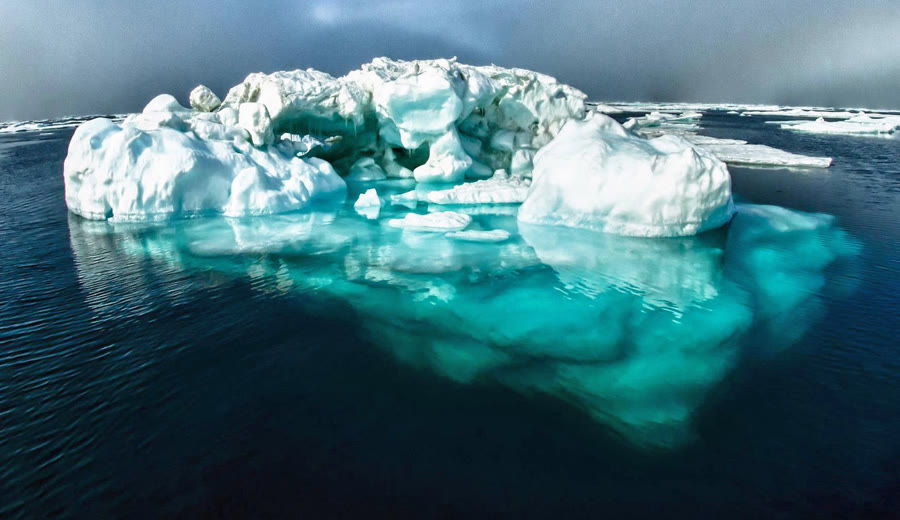
\includegraphics[width=0.66\linewidth]{images/book2/g11-noaa-iceberg.jpg}

{\small Gunung es yang dilihat dari tepat di atas air: es di bawah permukaan,
yang tampak menembus laut yang jernih, jauh lebih besar daripada bagian yang
berada di udara. Foto: NOAA (domain publik).}
\end{omfigure}
% ledger: photo:g11-iceberg

\section{Dua cara membagi Bumi menjadi lapisan}

Kerak, mantel, dan inti adalah lapisan-lapisan dari \emph{bahan} yang berbeda:
kerak terbuat dari batuan yang kaya akan silikon, aluminium, dan oksigen, mantel
dari batuan yang lebih rapat, inti dari logam. Tetapi bagian luar Bumi juga
dapat dibagi menurut \emph{perilaku} batuannya ketika gaya-gaya bekerja
padanya dalam waktu yang sangat lama.

\begin{definition}[Litosfer; astenosfer]\label{def:g11:lithosphere-asthenosphere:lithosphere}
Yang disebut \emph{litosfer}\index{litosfer} adalah kulit luar Bumi yang kaku:
kerak dan bagian mantel paling atas yang paling dingin, yang bersama-sama
terpecah menjadi lempeng-lempeng tektonik dan tidak mengalir. Yang disebut
\emph{astenosfer}\index{astenosfer} adalah lapisan mantel di bawah litosfer,
yang lebih panas dan lebih lemah, yang mengalir
perlahan-lahan dalam rentang waktu yang panjang, seperti pasta yang sangat kental.
\end{definition}

Batas antara keduanya terletak sekitar 70 sampai \qty{100}{km} di bawah
permukaan samudra dan kebanyakan benua, dan lebih dalam di bawah bagian benua
yang paling tua; di Amerika Serikat, misalnya, tebal \omterm{def:g11:lithosphere-asthenosphere:lithosphere}{litosfer} berkisar dari
sekitar \qty{40}{km} di barat sampai lebih dari \qty{200}{km} di bagian tengah
benua itu. Dasar \omterm{def:g11:lithosphere-asthenosphere:lithosphere}{litosfer} bukanlah \omterm{def:g11:seismic-structure:moho}{Moho}: sebagian besar \omterm{def:g11:lithosphere-asthenosphere:lithosphere}{litosfer} adalah batuan
mantel.
% ledger: rs09:lab, fischer:lab, porter:lab, usgs:lithosphere-80km (Book 1 row)

\begin{omfigure}
\begin{tikzpicture}[x=1cm, y=-0.0125cm, font=\footnotesize]
% depths to scale: crust 41 km (cm95:crust), lithosphere 100 km (rs09:lab), 0-400 km
  \shade[top color=omLithPeridotite!70, bottom color=omLithPeridotite!25] (5,100) rectangle (8,400);
  \fill[omLithGranite!55] (0,0) rectangle (3,41);
  \fill[omLithPeridotite!55] (0,41) rectangle (3,400);
  \fill[black!25] (5,0) rectangle (8,100);
  \draw (0,0) rectangle (3,400);
  \draw (5,0) -- (5,400) (8,0) -- (8,400) (5,0) -- (8,0);
  \draw[line width=0.8pt] (0,41) -- (3,41);
  \draw[line width=0.8pt, densely dashed] (5,100) -- (8,100);
  \draw[densely dotted, black!60] (3,41) -- (5,41);
  \node at (1.5,20) {kerak};
  \node[align=center] at (1.5,220) {mantel};
  \node[align=center] at (6.5,50) {litosfer\\kaku};
  \node[align=center] at (6.5,180) {astenosfer\\lemah, mengalir perlahan};
  \node[align=center, text=black!70] at (6.5,340) {mantel yang lebih dalam};
  \node[anchor=south, font=\small] at (1.5,0) {menurut bahan};
  \node[anchor=south, font=\small] at (6.5,0) {menurut perilaku};
  \foreach \d in {0,100,200,300,400} {\draw (-0.1,\d) -- (0,\d); \node[anchor=east] at (-0.1,\d) {\d};}
  \node[anchor=east, rotate=90, anchor=south] at (-0.9,200) {kedalaman (\unit{km})};
  \node[anchor=south, font=\scriptsize, align=center] at (4,41) {Moho\\(\qty{41}{km})};
  \node[anchor=west, align=left] at (8.15,100) {dasar\\litosfer\\(sekitar \qty{100}{km})};
\end{tikzpicture}

{\small Bagian Bumi setebal \qty{400}{km} yang paling atas di bawah sebuah benua,
dengan skala sebenarnya. Kiri: lapisan-lapisan menurut bahan. Kanan:
lapisan-lapisan menurut perilaku. \omterm{def:g11:lithosphere-asthenosphere:lithosphere}{Litosfer} yang kaku memuat seluruh kerak dan
bagian atas mantel; \omterm{def:g11:lithosphere-asthenosphere:lithosphere}{astenosfer} tidak mempunyai batas bawah yang tegas.}
\end{omfigure}

\section{Zona kecepatan rendah}

Gelombang seismik memperlihatkan \omterm{def:g11:lithosphere-asthenosphere:lithosphere}{astenosfer}. Hampir di mana-mana di Bumi,
kecepatan seismik bertambah seiring kedalaman, karena batuan makin lama makin
termampatkan. Di bawah \omterm{def:g11:lithosphere-asthenosphere:lithosphere}{litosfer}, yang terjadi justru sebaliknya.

\begin{definition}[Zona kecepatan rendah]\label{def:g11:lithosphere-asthenosphere:lvz}
Yang disebut \emph{zona kecepatan rendah}\index{zona kecepatan rendah} adalah
lapisan mantel atas, di bawah \omterm{def:g11:lithosphere-asthenosphere:lithosphere}{litosfer}, yang di dalamnya gelombang seismik
merambat lebih lambat daripada di batuan di atas dan di bawahnya.
\end{definition}

Dalam \omterm{def:g11:seismic-structure:reference-model}{model acuan Bumi}, kecepatan S turun perlahan dari \omterm{def:g11:seismic-structure:moho}{Moho} sampai
\qty{220}{km}, lalu melonjak naik. Studi seismik di seluruh dunia menemukan
penurunan kecepatan yang tajam di suatu tempat antara 70 dan \qty{100}{km}:
puncak \omterm{def:g11:lithosphere-asthenosphere:lithosphere}{astenosfer}. Batuan di sana cukup panas sehingga hampir meleleh, dan
mungkin mengandung sedikit sekali lelehan; batuan itu mungkin juga mengandung
lebih banyak air daripada batuan di atasnya. Batuan yang hampir meleleh itu
lemah: batuan itu memperlambat gelombang seismik, dan dapat mengalir.
% ledger: data:prem, rs09:lab, fischer:lab, porter:lab

\begin{omfigure}
\begin{tikzpicture}
\begin{axis}[omrecord, omdepth, width=0.6\linewidth, height=6.0cm, xmin=3.0, xmax=5.0, ymin=0, ymax=400,
  xlabel={kecepatan S (\unit{km/s})}, ylabel={kedalaman (\unit{km})}, xtick={3.0,3.5,...,5.0},
  xticklabel style={/pgf/number format/fixed, /pgf/number format/precision=1},
  tick label style={font=\small}, label style={font=\small}]
% computed in figdata/grade-11/prem_profiles.py (part upper); ledger: data:prem
\fill[black!10] (axis cs:3.0,80) rectangle (axis cs:5.0,220);
\addplot[omProp, line width=0.9pt] table[x=vs, y=depth] {figdata/out/grade-11-prem_profiles-upper.dat};
\node[font=\scriptsize, anchor=west, align=left] at (axis cs:3.1,150) {zona\\kecepatan rendah};
\node[font=\scriptsize, anchor=west] at (axis cs:3.95,12) {kerak};
\end{axis}
\end{tikzpicture}

{\small Kecepatan S pada \qty{400}{km} paling atas dalam \omterm{def:g11:seismic-structure:reference-model}{model acuan Bumi}. Di
bawah kerak, kecepatan itu berkurang perlahan seiring kedalaman sampai
\qty{220}{km} (diarsir mulai \qty{80}{km}), lalu bertambah lagi dengan
lompatan-lompatan mendadak.}
\end{omfigure}

\section{Geoterm}

\begin{definition}[Geoterm; gradien geotermal]\label{def:g11:lithosphere-asthenosphere:geotherm}
Yang disebut \emph{geoterm}\index{geoterm} adalah kurva suhu terhadap kedalaman
di bawah suatu tempat. Yang disebut
\emph{gradien geotermal}\index{gradien geotermal} adalah kenaikan suhu per satuan kedalaman, dalam derajat per kilometer.
\end{definition}

Lubang bor hanya mengukur \omterm{def:g11:lithosphere-asthenosphere:geotherm}{geoterm} pada beberapa kilometer pertama, tempat suhu
naik 25 sampai \qty{30}{\celsius} per kilometer (Buku 1, kelas 6). Lebih dalam
lagi, \omterm{def:g11:lithosphere-asthenosphere:geotherm}{geoterm} dihitung dari kalor yang mengalir keluar melalui permukaan dan
dari sifat-sifat batuan; \cref{ch:g12:internal-heat} menunjukkan dari mana kalor
itu berasal. Dua fakta membentuk hasilnya. Sebagian kalor dihasilkan di dalam
kerak atas itu sendiri, sehingga gradiennya paling curam di dekat permukaan dan
lebih kecil di bawah kerak. Dan di \omterm{def:g11:lithosphere-asthenosphere:lithosphere}{astenosfer}, yang mengalir, gerak lambat
batuan membawa kalor dan meratakan suhu: suhu hanya naik sekitar
\qty{0.45}{\celsius} per kilometer. Dasar \omterm{def:g11:lithosphere-asthenosphere:lithosphere}{litosfer} ditempatkan di tempat \omterm{def:g11:lithosphere-asthenosphere:geotherm}{geoterm}
\omterm{def:g11:lithosphere-asthenosphere:lithosphere}{litosfer} yang curam bertemu dengan \omterm{def:g11:lithosphere-asthenosphere:geotherm}{geoterm} \omterm{def:g11:lithosphere-asthenosphere:lithosphere}{astenosfer} yang landai, pada sekitar
\qty{1300}{\celsius}.
% ledger: usgs:gradient-29 (Book 1 row), b2dd10:continents, b2roy:provinces, roy:conductivity,
% katsura10:adiabat, porter:lab

\begin{omfigure}
\begin{tikzpicture}
\begin{axis}[omrecord, omdepth, width=0.7\linewidth, height=6.4cm, xmin=0, xmax=2000, ymin=0, ymax=300,
  xlabel={suhu (\unit{\celsius})}, ylabel={kedalaman (\unit{km})}, xtick={0,500,...,2000},
  tick label style={font=\small}, label style={font=\small}]
% computed in figdata/grade-11/geotherm_solidus.py; ledger: b2dd10:continents, b2roy:provinces,
% roy:conductivity, porter:lab, katsura10:adiabat, hirschmann:solidus, data:prem
\fill[black!8] (axis cs:0,99.7) rectangle (axis cs:2000,300);
\addplot[omDef, line width=1.0pt] table[x=t_geotherm, y=depth_km] {figdata/out/grade-11-geotherm_solidus-geotherm.dat};
\addplot[omDef, densely dashed, restrict y to domain=99:300] table[x=t_cond, y=depth_km] {figdata/out/grade-11-geotherm_solidus-geotherm.dat};
\addplot[omProp, line width=1.0pt] table[x=t_solidus, y=depth_km] {figdata/out/grade-11-geotherm_solidus-geotherm.dat};
\draw[black!60] (axis cs:0,99.7) -- (axis cs:2000,99.7);
\node[font=\scriptsize, anchor=south west] at (axis cs:20,99.7) {dasar litosfer};
\node[font=\scriptsize, anchor=north west] at (axis cs:20,102) {astenosfer};
\node[font=\scriptsize, text=omDef, anchor=north west] at (axis cs:480,6) {geoterm};
\node[font=\scriptsize, text=omProp, anchor=west] at (axis cs:1300,22) {pelelehan mulai};
\end{axis}
\end{tikzpicture}

{\small \omterm{def:g11:lithosphere-asthenosphere:geotherm}{Geoterm} model di bawah sebuah benua (biru) dan suhu tempat batuan mantel
(peridotit, tanpa air) mulai meleleh (jingga). \omterm{def:g11:lithosphere-asthenosphere:geotherm}{Geoterm} itu dihitung dari aliran
kalor rata-rata benua-benua dan sifat batuan yang terukur; di \omterm{def:g11:lithosphere-asthenosphere:lithosphere}{astenosfer}
(kelabu) \omterm{def:g11:lithosphere-asthenosphere:geotherm}{geoterm} naik perlahan. Garis putus-putus menunjukkan bagaimana kenaikan
\omterm{def:g11:lithosphere-asthenosphere:lithosphere}{litosfer} yang lebih curam akan berlanjut. Kedua kurva paling berdekatan, dengan
selisih sekitar \qty{140}{\celsius}, di dekat dasar \omterm{def:g11:lithosphere-asthenosphere:lithosphere}{litosfer}.}
\end{omfigure}
% values: lab_km 99.7, t_lab_c 1345, closest_gap_c 144 (figdata/grade-11/geotherm_solidus.py)

Suhu leleh batuan mantel naik seiring kedalaman, karena batuan makin lama makin
termampatkan (Buku 1, kelas 6): sekitar \qty{1120}{\celsius} di permukaan,
hampir \qty{1500}{\celsius} pada \qty{100}{km}. Dalam model itu, \omterm{def:g11:lithosphere-asthenosphere:geotherm}{geoterm} paling
mendekati suhu leleh tepat di bawah \omterm{def:g11:lithosphere-asthenosphere:lithosphere}{litosfer}, sekitar \qty{140}{\celsius} di
bawahnya. Sedikit air, atau mantel yang sedikit lebih panas, menutup selisih
itu: di bagian barat Amerika Serikat, tempat \omterm{def:g11:lithosphere-asthenosphere:lithosphere}{litosfer} tipis, sebagian kecil
mantel di bawahnya meleleh sebagian.
% ledger: hirschmann:solidus, porter:lab; computed in figdata/grade-11/geotherm_solidus.py
% (solidus0_c 1120.7, solidus100_c 1489, closest_gap_c 144)

\section{Isostasi}

\subsection{Mengapung di atas zat padat}

Selama beberapa detik perambatan gelombang gempa bumi, \omterm{def:g11:lithosphere-asthenosphere:lithosphere}{astenosfer} adalah zat
padat. Dalam rentang waktu yang panjang, \omterm{def:g11:lithosphere-asthenosphere:lithosphere}{astenosfer} mengalir. Beban yang
diletakkan di atas \omterm{def:g11:lithosphere-asthenosphere:lithosphere}{litosfer} --- jajaran pegunungan, lapisan es --- perlahan-lahan
mendesak \omterm{def:g11:lithosphere-asthenosphere:lithosphere}{astenosfer} ke samping sampai beban itu mengapung, seperti balok kayu di
atas air.

\begin{definition}[Isostasi; kedalaman kompensasi]\label{def:g11:lithosphere-asthenosphere:isostasy}
Yang disebut \emph{isostasi}\index{isostasi} adalah keseimbangan yang membuat
lapisan-lapisan luar Bumi mengapung di atas \omterm{def:g11:lithosphere-asthenosphere:lithosphere}{astenosfer}: pada suatu kedalaman di
mantel yang disebut \emph{kedalaman kompensasi}\index{kedalaman kompensasi},
setiap kolom batuan dengan penampang yang sama, dari permukaan sampai kedalaman
itu, mempunyai berat yang sama, apa pun relief di atasnya.
\end{definition}

\begin{omfigure}
\begin{tikzpicture}[x=1cm, y=1cm, font=\footnotesize, >={Stealth[length=4pt]}]
% not to scale
  \fill[omSea!50] (6,0) rectangle (8.6,-0.9);
  \fill[omLithPeridotite!45] (0,-5.2) rectangle (2.6,-6.6);
  \fill[omLithGranite!55] (0,2.0) -- (2.6,2.0) -- (2.6,-5.2) -- (0,-5.2) -- cycle;
  \fill[omLithGranite!55] (2.6,0) rectangle (6,-3.0);
  \fill[omLithGranite!55] (6,-0.9) rectangle (8.6,-1.6); % same fill: one crustal density in Airy's model
  \fill[omLithPeridotite!45] (2.6,-3.0) rectangle (6,-6.6);
  \fill[omLithPeridotite!45] (6,-1.6) rectangle (8.6,-6.6);
  \draw (0,2.0) -- (2.6,2.0) -- (2.6,0) -- (6,0);
  \draw (6,0) -- (8.6,0);
  \draw[line width=0.8pt] (0,-5.2) -- (2.6,-5.2) -- (2.6,-3.0) -- (6,-3.0) -- (6,-1.6) -- (8.6,-1.6);
  \draw[densely dashed, line width=0.8pt] (0,-6.2) -- (8.6,-6.2);
  \node[anchor=north east] at (8.6,-6.6) {kedalaman kompensasi};
  \draw[black!50, densely dotted] (-0.2,0) -- (0,0);
  \node[anchor=east] at (-0.2,0) {permukaan laut};
  \node at (1.3,-1.6) {kerak};
  \node at (4.3,-1.5) {kerak};
  \node at (7.3,-0.45) {samudra};
  \node at (7.3,-1.25) {kerak};
  \node at (4.3,-4.8) {mantel};
  \node[anchor=south] at (1.3,2.0) {jajaran pegunungan};
  \node[anchor=south] at (4.3,0) {dataran rendah};
  \draw[<->] (2.75,0) -- (2.75,2.0); \node[anchor=west] at (2.8,1.0) {$h$};
  \draw[<->] (2.75,-3.0) -- (2.75,-5.2); \node[anchor=west] at (2.8,-4.1) {akar $r$};
  \draw[<->] (5.85,0) -- (5.85,-3.0); \node[anchor=east] at (5.8,-1.0) {$T$};
\end{tikzpicture}

{\small Model \omterm{prop:g11:lithosphere-asthenosphere:airy}{isostasi Airy} (tidak berskala). Massa jenis kerak sama di
mana-mana; di tempat kerak itu menjulang tinggi, kerak itu tebal dan mempunyai
akar yang menjangkau jauh ke dalam mantel yang lebih rapat. Di bawah samudra,
kerak itu tipis. Ketiga kolom itu sama beratnya sampai \omterm{def:g11:lithosphere-asthenosphere:isostasy}{kedalaman kompensasi}.}
\end{omfigure}

\subsection{Akar jajaran pegunungan}

\begin{proposition}[Isostasi Airy]\label{prop:g11:lithosphere-asthenosphere:airy}
Misalkan kerak mempunyai massa jenis seragam $\rho_c$, dan mantel di bawahnya
mempunyai massa jenis $\rho_m > \rho_c$. Jika suatu wilayah menjulang setinggi
$h$ di atas wilayah lain dan keduanya berada dalam keseimbangan isostatik,
keraknya lebih tebal sebesar
\[
  \Delta H = h\,\frac{\rho_m}{\rho_m - \rho_c},
\]
dengan $h$ menjulang di atas wilayah lain itu dan akar
$r = h\,\rho_c/(\rho_m - \rho_c)$ menjangkau ke bawah keraknya.\index{isostasi Airy}
\end{proposition}

\begin{proof}
Ambillah dua kolom dengan luas $S$ yang sama, dataran rendah dengan kerak
setebal $T$ dan jajaran pegunungan, yang keraknya menjulang $h$ lebih tinggi dan
menjangkau $r$ lebih dalam, sehingga tebalnya $T + h + r$. Sampai \omterm{def:g11:lithosphere-asthenosphere:isostasy}{kedalaman
kompensasi} di bawah kedua \omterm{def:g11:seismic-structure:moho}{Moho}, kolom pegunungan mempunyai kerak $h + r$ lebih
banyak; sebagai gantinya, kolom dataran rendah mempunyai mantel setebal $r$.
Dengan $g$ percepatan gravitasi, kedua berat itu sama bila
\[
  \rho_c\,(h + r)\,S\,g = \rho_m\,r\,S\,g,
  \qquad\text{yaitu}\qquad
  r = h\,\frac{\rho_c}{\rho_m - \rho_c}.
\]
Kerak lebih tebal sebesar $h + r = h\,\bigl(1 + \rho_c/(\rho_m - \rho_c)\bigr)
= h\,\rho_m/(\rho_m - \rho_c)$.
\end{proof}

Dengan massa jenis rata-rata kerak benua, $\rho_c =
\qty{2830}{kg/m^3}$, dan massa jenis mantel tepat di bawah \omterm{def:g11:seismic-structure:moho}{Moho}, $\rho_m =
\qty{3380}{kg/m^3}$, akarnya $2830/550 \approx 5.1$ kali tingginya, dan kerak
lebih tebal sekitar $6.1$ kali tingginya: jajaran pegunungan yang menjulang
\qty{3}{km} di atas sekelilingnya mempunyai akar sekitar \qty{15}{km}.
% ledger: cm95:crust, data:prem (rho 3.38 below the Moho)

\begin{method}[Menghitung akar]\label{met:g11:lithosphere-asthenosphere:root}
\begin{enumerate}
  \item Tentukan tinggi $h$ wilayah itu di atas wilayah acuan yang tebal
        keraknya diketahui.
  \item Hitung $\rho_m/(\rho_m - \rho_c)$ dengan massa jenis kerak dan
        mantel.
  \item Kerak lebih tebal daripada kerak acuan sebesar $h\,\rho_m/(\rho_m -
        \rho_c)$; akarnya saja sama dengan nilai itu dikurangi $h$.
\end{enumerate}
\end{method}

\begin{example}[Dataran tinggi setinggi \qty{2}{km}]\label{ex:g11:lithosphere-asthenosphere:plateau}
Sebuah dataran tinggi menjulang \qty{2}{km} di atas dataran rendah yang keraknya
setebal \qty{37}{km}. Keraknya lebih tebal sebesar
$2 \times 3380/550 \approx \qty{12.3}{km}$: seluruhnya sekitar \qty{49}{km},
dengan akar sekitar \qty{10}{km}.
\end{example}

\subsection{Mengapa benua menjulang tinggi}

\begin{definition}[Kurva hipsometri]\label{def:g11:lithosphere-asthenosphere:hypsometry}
Yang disebut \emph{kurva hipsometri}\index{kurva hipsometri} Bumi adalah kurva
yang memberikan, untuk setiap ketinggian, bagian permukaan Bumi yang terletak
lebih tinggi daripadanya. Kemiringannya menunjukkan seberapa banyak permukaan
yang terletak pada setiap ketinggian.
\end{definition}

Jika permukaan itu dibentuk secara kebetulan, sebagian besarnya akan terletak di
dekat satu aras rata-rata. Kenyataannya tidak begitu.

\begin{proposition}[Dua aras]\label{prop:g11:lithosphere-asthenosphere:two-levels}
Ketinggian permukaan Bumi mengelompok di sekitar dua aras: satu dalam selisih
beberapa ratus meter dari permukaan laut, di benua-benua, dan satu sekitar 4
sampai \qty{5}{km} di bawah permukaan laut, di dasar samudra dalam. Daratan
meliputi \qty{29}{\percent} permukaan; lebih dari separuh permukaan terletak
lebih dalam daripada \qty{3}{km} di bawah permukaan laut, dan hanya
\qty{3}{\percent} yang menjulang lebih tinggi daripada \qty{2}{km}.
\end{proposition}
% computed in figdata/grade-11/hypsometry.py from ETOPO1 (land_fraction 0.290,
% share_below_3000_pct 53.4, share_above_2000_pct 3.1; modes at +250 and -4250 m); ledger: data:etopo1

\begin{omfigure}
\begin{tikzpicture}
\begin{axis}[omrecord, width=0.86\linewidth, height=5.4cm, xmin=-11000, xmax=9000, ymin=0, ymax=18,
  xlabel={ketinggian (\unit{m}; negatif: di bawah permukaan laut)}, ylabel={bagian permukaan (\unit{\percent})},
  xtick={-10000,-8000,...,8000}, scaled x ticks=false, xticklabel style={/pgf/number format/1000 sep={\,}, font=\scriptsize},
  tick label style={font=\small}, label style={font=\small}, clip=false]
% computed in figdata/grade-11/hypsometry.py; ledger: data:etopo1
\addplot[ybar interval, fill=omSea!70, draw=black!50, restrict expr to domain={\thisrow{land}}{0:0}] table[x=lo, y=share_pct] {figdata/out/grade-11-hypsometry-bins.dat};
\addplot[ybar interval, fill=omHypsLandC, draw=black!50, restrict expr to domain={\thisrow{land}}{1:1}] table[x=lo, y=share_pct] {figdata/out/grade-11-hypsometry-bins.dat};
\draw[black!60, densely dotted] (axis cs:0,0) -- (axis cs:0,18);
\node[font=\scriptsize, anchor=south west] at (axis cs:600,15.5) {benua};
\node[font=\scriptsize, anchor=south] at (axis cs:-4250,12.2) {dasar samudra dalam};
\end{axis}
\end{tikzpicture}

{\small Bagian permukaan Bumi pada setiap pita ketinggian selebar \qty{500}{m}
(dari ETOPO1, dengan resolusi satu derajat; di atas Antarktika dan Greenland,
permukaan esnya). Kedua puncak itu adalah benua-benua dan dasar samudra dalam.}
\end{omfigure}

\omterm{def:g11:lithosphere-asthenosphere:isostasy}{Isostasi} menjelaskan kedua aras itu. Benua terbuat dari kerak yang tebal,
rata-rata sekitar \qty{41}{km}, dari batuan yang ringan; dasar samudra dari
kerak tipis dari batuan yang lebih rapat, yang tebalnya hanya sekitar
\qty{5}{km}. Keduanya mengapung di atas \omterm{def:g11:lithosphere-asthenosphere:lithosphere}{astenosfer}: kerak benua yang tebal dan
ringan mengapung tinggi, kerak samudra yang tipis dan rapat mengapung rendah, dan
samudra mengisi tanah yang rendah itu.
% ledger: cm95:crust, usgs:crust-thickness (Book 1 row)

\section{Tutup yang lentur}

\omterm{def:g11:lithosphere-asthenosphere:isostasy}{Isostasi} memerlukan \omterm{def:g11:lithosphere-asthenosphere:lithosphere}{astenosfer} yang mengalir. \omterm{def:g11:lithosphere-asthenosphere:lithosphere}{Litosfer} di atasnya tidak
mengalir; \omterm{def:g11:lithosphere-asthenosphere:lithosphere}{litosfer} itu melentur. Beban yang lebih sempit daripada tebal
\omterm{def:g11:lithosphere-asthenosphere:lithosphere}{litosfer}, seperti satu pulau gunung api, ditopang oleh kekakuan lempeng, seperti
pemberat di atas papan, dan lempeng itu melendut di sekelilingnya. Beban yang
jauh lebih lebar daripada tebal itu, seperti seluruh jajaran pegunungan atau
lapisan es, tenggelam sampai mengapung. Bila beban itu disingkirkan, \omterm{def:g11:lithosphere-asthenosphere:lithosphere}{litosfer}
perlahan-lahan naik lagi (\cref{ch:g12:destruction-of-mountains}).

\section{Latihan}

\begin{exercise}[$\star$]\label{exo:g11:lithosphere-asthenosphere:1}
Definisikan \omterm{def:g11:lithosphere-asthenosphere:lithosphere}{litosfer} dan \omterm{def:g11:lithosphere-asthenosphere:lithosphere}{astenosfer}. Manakah di antara yang berikut ini yang
termasuk \omterm{def:g11:lithosphere-asthenosphere:lithosphere}{litosfer}: kerak samudra, kerak benua, mantel paling atas, inti luar?
\end{exercise}

\begin{exercise}[$\star$]\label{exo:g11:lithosphere-asthenosphere:2}
Sebuah gunung es dengan massa jenis \qty{910}{kg/m^3} mengapung di air laut
dengan massa jenis \qty{1025}{kg/m^3}. Berapa bagian volumenya yang terletak di
bawah air? Jika sebuah gunung es bersisi tegak menjulang \qty{20}{m} di atas air,
berapa tinggi totalnya?
\end{exercise}

\begin{exercise}[$\star$]\label{exo:g11:lithosphere-asthenosphere:3}
Suhu tanah \qty{15}{\celsius} dan \omterm{def:g11:lithosphere-asthenosphere:geotherm}{gradien geotermalnya}
\qty{26}{\celsius} per kilometer. Berapa suhu di dasar lubang bor sedalam
\qty{3}{km}? Mengapa gradien yang sama tidak dapat dipakai sampai
\qty{100}{km}?
\end{exercise}

\begin{exercise}[$\star$]\label{exo:g11:lithosphere-asthenosphere:4}
Dari gambar ketinggian permukaan Bumi, berikan dua pita ketinggian yang paling
umum dan bagian permukaan pada masing-masing pita itu.
\end{exercise}

\begin{exercise}[$\star$]\label{exo:g11:lithosphere-asthenosphere:5}
Dengan rumus $T = -5.104\,P^2 + 132.899\,P + 1120.661$ (suhu dalam
\unit{\celsius}, tekanan $P$ dalam gigapascal), hitung suhu tempat batuan
mantel kering mulai meleleh di permukaan ($P = 0$) dan pada
\qty{3}{GPa}, sekitar \qty{95}{km} di bawah permukaan.
\end{exercise}

\begin{exercise}[$\star\star$]\label{exo:g11:lithosphere-asthenosphere:6}
Pada gambar \omterm{def:g11:lithosphere-asthenosphere:geotherm}{geoterm} model, baca suhu pada 50, 150, dan
\qty{250}{km}. Di lapisan mana, \omterm{def:g11:lithosphere-asthenosphere:lithosphere}{litosfer} atau \omterm{def:g11:lithosphere-asthenosphere:lithosphere}{astenosfer}, setiap kedalaman itu
berada? Di antara dua kedalaman yang mana suhu naik paling banyak?
\end{exercise}

\begin{exercise}[$\star\star$]\label{exo:g11:lithosphere-asthenosphere:7}
Sebuah jajaran pegunungan menjulang \qty{3}{km} di atas dataran rendah; ambillah
$\rho_c =
\qty{2830}{kg/m^3}$ dan $\rho_m = \qty{3380}{kg/m^3}$. Hitung akarnya dan
tambahan tebal keraknya.
\end{exercise}

\begin{exercise}[$\star\star$]\label{exo:g11:lithosphere-asthenosphere:8}
Suatu wilayah mempunyai kerak setebal \qty{55}{km}. Dengan massa jenis pada
\cref{exo:g11:lithosphere-asthenosphere:7}, setinggi apa wilayah itu menjulang
di atas wilayah yang keraknya setebal \qty{41.1}{km}?
\end{exercise}

\begin{exercise}[$\star\star$]\label{exo:g11:lithosphere-asthenosphere:9}
Dalam model acuan, kecepatan S adalah \qty{4.470}{km/s} pada \qty{80}{km},
\qty{4.419}{km/s} tepat di atas \qty{220}{km}, dan \qty{4.644}{km/s} tepat di
bawahnya. Hitung, dalam persen, penurunan antara 80 dan \qty{220}{km} dan
lonjakan pada \qty{220}{km}. Mengapa penurunan kecepatan seiring kedalaman itu
mengejutkan?
\end{exercise}

\begin{exercise}[$\star\star$]\label{exo:g11:lithosphere-asthenosphere:10}
Dalam \omterm{def:g11:lithosphere-asthenosphere:geotherm}{geoterm} model, suhunya \qty{610}{\celsius} di \omterm{def:g11:seismic-structure:moho}{Moho}, pada kedalaman
\qty{40}{km}, dan \qty{1345}{\celsius} di dasar \omterm{def:g11:lithosphere-asthenosphere:lithosphere}{litosfer}, pada kedalaman
\qty{100}{km}. (1) Hitung gradien rata-rata di antara keduanya. (2)
Bandingkan dengan gradien di permukaan, \qty{26}{\celsius} per kilometer,
dan jelaskan perbedaannya.
\end{exercise}

\begin{exercise}[$\star\star$]\label{exo:g11:lithosphere-asthenosphere:11}
Di \omterm{def:g11:lithosphere-asthenosphere:lithosphere}{astenosfer} suhu dianggap sama dengan $1300 + 0.45\,z$ (dalam
\unit{\celsius}, $z$ dalam kilometer). Hitung suhu itu pada 200 dan \qty{400}{km}.
Berapa kenaikannya di antara keduanya? Bandingkan dengan kenaikan pada
\qty{100}{km} pertama, dari \qty{15}{\celsius} di permukaan sampai
\qty{1345}{\celsius} di dasar \omterm{def:g11:lithosphere-asthenosphere:lithosphere}{litosfer}.
\end{exercise}

\begin{exercise}[$\star\star\star$]\label{exo:g11:lithosphere-asthenosphere:12}
Di bawah kerak atas, \omterm{def:g11:lithosphere-asthenosphere:geotherm}{geoterm} model mendekati $T \approx 118 +
G\,z$ (dalam \unit{\celsius}, $z$ dalam kilometer), dengan gradien $G$ yang
bergantung pada kalor yang datang dari bagian yang lebih dalam. (1) Untuk $G =
\qty{12.3}{\celsius}$ per kilometer, seperti yang dihitung untuk bagian timur
Amerika Serikat, tentukan kedalaman tempat \omterm{def:g11:lithosphere-asthenosphere:geotherm}{geoterm} itu bertemu dengan
$1300 + 0.45\,z$. (2) Lakukan hal yang sama untuk $G = \qty{21.5}{\celsius}$
per kilometer, seperti yang dihitung untuk provinsi
Cekungan dan Pegunungan di barat.
(3) Bandingkan dengan tebal yang terukur, dari sekitar \qty{40}{km} di barat
sampai lebih dari \qty{200}{km} di bagian tengah benua itu.
\end{exercise}

\begin{exercise}[$\star\star\star$]\label{exo:g11:lithosphere-asthenosphere:13}
(1) Tunjukkan bahwa, dalam model Airy, wilayah yang keraknya $\Delta H$ lebih
tebal daripada wilayah acuan menjulang lebih tinggi sebesar
$\Delta H\,(\rho_m - \rho_c)/\rho_m$. (2) Berapa bagian dari setiap tambahan
tebal kerak yang tampak sebagai ketinggian? (3) Bandingkan dengan bagian gunung
es yang menjulang di atas air.
\end{exercise}

\begin{exercise}[$\star\star\star$]\label{exo:g11:lithosphere-asthenosphere:14}
Pada \qty{100}{km} batuan mantel kering mulai meleleh pada \qty{1489}{\celsius},
dan \omterm{def:g11:lithosphere-asthenosphere:geotherm}{geoterm} model berada pada \qty{1345}{\celsius}. (1) Berapa derajat air harus
menurunkan suhu leleh agar batuan itu mulai meleleh di sana? (2) Mengapa bahkan
bagian lelehan yang sangat kecil membuat batuan itu lemah dan memperlambat
gelombang seismik?
\end{exercise}

\begin{exercise}[$\star\star\star$]\label{exo:g11:lithosphere-asthenosphere:15}
Hanya \qty{3}{\percent} permukaan Bumi yang menjulang di atas \qty{2}{km},
sedangkan \qty{53}{\percent} terletak lebih dari \qty{3}{km} di bawah permukaan
laut. (1) Jika seluruh daratan diratakan dan batuannya dibuang ke samudra,
apakah permukaan itu akhirnya berada di dekat permukaan laut? Gunakan \omterm{def:g11:lithosphere-asthenosphere:isostasy}{isostasi}
untuk menjelaskan jawabanmu. (2) Apa yang disampaikan oleh adanya dua aras itu
tentang kerak?
\end{exercise}

\section{Soal: Mengapa Tibet Menjulang Lima Kilometer}

\begin{problem}[{Soal akhir pekan --- menimbang sebuah dataran tinggi}]
\label{pb:g11:lithosphere-asthenosphere:1}
% values computed in figdata/grade-11/hypsometry.py (tibet_mean_m 5015, qaidam_mean_m 3230,
% mean_land_no_antarctica_m 674); ledger: data:etopo1, cm95:crust, data:prem, karplus:tibet-moho
Dataran tinggi Tibet adalah wilayah tinggi yang terbesar di Bumi. Di antara
lintang \ang{31} dan \ang{35} LU dan bujur \ang{80} dan \ang{95} BT,
ketinggian rata-ratanya \qty{5010}{m}; ketinggian rata-rata seluruh daratan di
luar Antarktika adalah \qty{670}{m}. Kerak benua rata-rata setebal
\qty{41.1}{km} dan mempunyai massa jenis rata-rata $\rho_c = \qty{2830}{kg/m^3}$;
mantel tepat di bawah \omterm{def:g11:seismic-structure:moho}{Moho} mempunyai massa jenis $\rho_m = \qty{3380}{kg/m^3}$.

\medskip
\noindent\textbf{Bagian I --- Dataran tinggi dan benua rata-rata.}
\begin{enumerate}
  \item Berapa lebih tinggi dataran tinggi itu menjulang daripada benua rata-rata?
  \item Berapa persen massa jenis kerak lebih kecil daripada mantel di bawahnya?
  \item Balok kerak yang mengapung bebas di atas batuan mantel akan tenggelam
        sampai berapa bagian tebalnya terletak di bawah permukaan mantel?
        Bandingkan dengan gunung es ($910$ dalam $1025$).
  \item Mantel itu padat. Dalam rentang waktu yang mana mantel berperilaku
        sebagai zat padat, dan dalam rentang waktu yang mana mantel dapat
        berperilaku seperti air di sekeliling gunung es?
  \item Mengapa \omterm{def:g11:lithosphere-asthenosphere:isostasy}{kedalaman kompensasi} harus dipilih di bawah \omterm{def:g11:seismic-structure:moho}{Moho} kedua
        kolom?
\end{enumerate}

\medskip
\noindent\textbf{Bagian II --- Keseimbangan Airy untuk dua kolom.}
\begin{enumerate}[resume]
  \item Gambarlah kedua kolom itu, benua rata-rata dan dataran tinggi, dari
        permukaannya sampai kedalaman \qty{70}{km} di bawah permukaan laut,
        dengan kerak dataran tinggi lebih tebal sebesar $\Delta H$.
  \item Tuliskan bahwa kedua kolom itu sama beratnya, dan simpulkan $\Delta H$
        dalam selisih ketinggian $h$ dan massa jenis.
  \item Hitung $\rho_m/(\rho_m - \rho_c)$.
  \item Hitung akar dataran tinggi itu di bawah \omterm{def:g11:seismic-structure:moho}{Moho} benua
        rata-rata.
  \item Berapa kedalaman \omterm{def:g11:seismic-structure:moho}{Moho} benua rata-rata di bawah permukaan laut, dan
        berapa kedalaman \omterm{def:g11:seismic-structure:moho}{Moho} dataran tinggi itu?
\end{enumerate}

\medskip
\noindent\textbf{Bagian III --- Tebal kerak.}
\begin{enumerate}[resume]
  \item Hitung tebal kerak di bawah dataran tinggi itu.
  \item Periksa keseimbangannya: hitung, untuk setiap kolom, massa batuan di
        atas satu meter persegi sampai \qty{70}{km} di bawah permukaan laut,
        dalam ton.
  \item Berapa tebal kerak di bawah dataran rendah pada permukaan laut?
  \item Berapa kali lebih tebal kerak di bawah Tibet daripada kerak benua
        rata-rata?
  \item Jika mantel sedikit lebih ringan, $\rho_m = \qty{3300}{kg/m^3}$,
        tebal berapa yang akan diberikan model itu? Apakah hasilnya sangat
        peka terhadap massa jenis?
\end{enumerate}

\medskip
\noindent\textbf{Bagian IV --- Perbandingan dengan pengukuran seismik.}
\begin{enumerate}[resume]
  \item Gelombang seismik yang terkonversi di \omterm{def:g11:seismic-structure:moho}{Moho} menempatkannya sekitar
        \qty{70}{km} di bawah permukaan Tibet utara. Bandingkan dengan pertanyaan~11.
  \item Tepat di utara dataran tinggi itu, cekungan Qaidam terletak pada
        ketinggian rata-rata \qty{3230}{m}, dan \omterm{def:g11:seismic-structure:moho}{Moho-nya} terletak sekitar
        \qty{50}{km} di bawah permukaan. Tebal kerak berapa yang diramalkan
        model Airy di sana?
  \item Cekungan Qaidam terisi sedimen setebal beberapa kilometer, yang lebih
        ringan daripada kerak rata-rata. Apakah hal itu membuat kerak yang
        sebenarnya lebih tipis atau lebih tebal daripada kerak model? Jelaskan.
  \item Sifat \omterm{def:g11:lithosphere-asthenosphere:lithosphere}{astenosfer} apa yang memungkinkan keseimbangan seperti itu?
  \item Simpulkan: berapa tebal kerak di bawah Tibet, dan mengapa dataran tinggi
        itu menjulang lima kilometer?
\end{enumerate}
\end{problem}
